\documentclass{article}
\usepackage{amsmath}
\usepackage{graphicx}
\begin{document}
\title{Equations of Lines: Question 12}
\author{Ana Bhattacharjee}
\date{\today}
\maketitle{}

\begin{center}
The image of the square is shown below.
\begin{figure}
  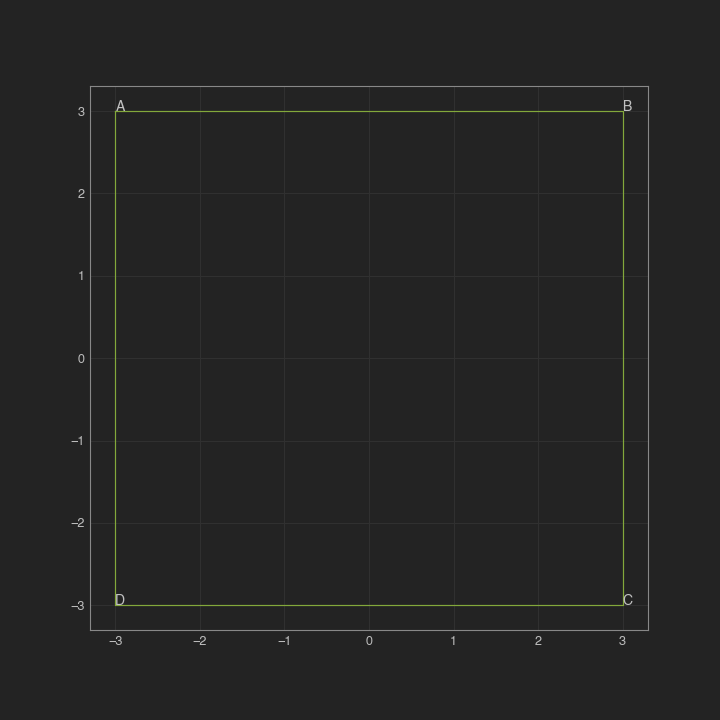
\includegraphics[width=1.1\columnwidth]{../line_eq_q12}
  \caption{Square with Diagonals}
\end{figure}
The steps for calculating the two equations of the diagonals are as follows:
\begin{itemize}
  \item Find the slope of one diagonal .
  \item Find the equation of one diagonal.
  \item Divide -1 by the slope to get the other diagonal's slope
  \item Find the equation of the other diagonal.
\end{itemize}
\par
\begin{align}
  A (-3, 3) \\
  C (3, -3) \\
  B (3,3) \\
  D (-3, -3) \\
  \text{slope\_{AC}} = \frac{3 - (-3)}{-3 - 3} \rightarrow \frac{6}{-6} = -1 \\
  \text{slope\_{BD}} = -1 x = -1 \rightarrow x = \frac{-1}{-1} = 1 \\
  y = mx + b \\
  3 = -1(-3) + b \rightarrow b = 0 \\
  -3 = -3(1) + b \rightarrow b = 0 \\
  AC \rightarrow y = -x \\
  BD \rightarrow y = x
\end{align}
\end{center}
\end{document}
